\documentclass{article}
\usepackage{dipole}
%\usepackage{showkeys}

\begin{document}
\title{Bipolar comparison}
\author{Nina Lebedeva, Anton Petrunin and Vladimir Zolotov}

\nofootnote{The first author was partially supported by RFBR grant 17-01-00128, 
the second author was partially supported by NSF grant DMS 1309340,
the third author was supported in part by DFG grant SPP 2026 and RFBR grant 17-01-00128.}


\newcommand{\Addresses}{{\bigskip\footnotesize

  Nina Lebedeva, \par\nopagebreak
  \textsc{Steklov Institute,
27 Fontanka, St. Petersburg, 
191023, Russia.}
  \par\nopagebreak\textsc{Math. Dept.
St. Petersburg State University,
Universitetsky pr., 28, 
Stary Peterhof, 
198504, Russia.}
  \par\nopagebreak
  \textit{Email}: \texttt{lebed@pdmi.ras.ru}

\medskip

  Anton Petrunin, \par\nopagebreak\textsc{Math. Dept. PSU, University Park, PA 16802, USA}
  \par\nopagebreak
  \textit{Email}: \texttt{petrunin@math.psu.edu}
  
\medskip

Vladimir Zolotov, \par\nopagebreak\textsc{Steklov Institute,
27 Fontanka, St. Petersburg, 
191023, Russia.}
  \par\nopagebreak
  \textsc{Math. Dept.
St. Petersburg State University,
Universitetsky pr., 28, 
Stary Peterhof, 
198504, Russia.}
  \par\nopagebreak
  \textit{Email}: \texttt{paranuel@mail.ru}
}}

\date{}

\maketitle

\begin{abstract}
We define the so called tree comparison --- a type of metric comparison which generalize the Alexandrov comparison and defined in a similar fashion.
This type of comparison turns out to have strong connections to continuity of optimal transport between regular measures on a Riemannian manifold, in particular to the so called MTW condition introduced by Xi-Nan Ma, Neil Trudinger and Xu-Jia Wang.

\end{abstract}

\section{Introduction}\label{sec:intro}

We will denote by $|a-b|_X$ the distance between points $a$ and $b$ in the metric space $X$.

\parbf{Tree comparison.}
Fix a tree $T$ with $n$ vertexes.

Let $(a_1,\dots a_n)$ be a point array in a metric space $X$ labeled by the vertexes of $T$.
We say that $(a_1,\dots a_n)$  satisfies the \emph{$T$-tree comparison} if there is a point array $(\~a_1,\dots, \~a_n)$ in the Hilbert space $\HH$ such that 
\[|\~a_i-\~a_j|_\HH\ge|a_i-a_j|_X\]
for any $i$ and $j$ and the equality holds if $a_i$ and $a_j$ are adjacent in $T$.

We say that a metric space $X$ satisfies the \emph{$T$-tree comparison} if 
every $n$-points array in $X$ satisfies the $T$-tree comparison.

Instead of the Hilbert space $\HH$ we may use infinite dimensional sphere or infinite dimensional hyperbolic space.
In this case we will it defines \emph{spherical} and \emph{hyperbolic} tree comparisons.

\hide
\begin{wrapfigure}{r}{27 mm}
\vskip-8mm
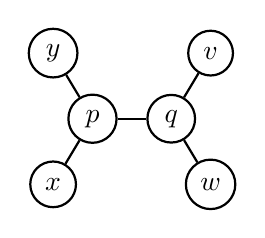
\begin{tikzpicture}[scale=1,
  thick,main node/.style={circle,draw,font=\sffamily\bfseries,minimum size=3mm}]
  \node[main node] (1) at (-1/2,-5/6) {$x$};
  \node[main node] (2) at (0,0){$p$};
  \node[main node] (3) at (-1/2,5/6){$y$};
  \node[main node] (4) at (3/2,5/6) {$v$};
  \node[main node] (5) at (1,0) {$q$};
  \node[main node] (6) at (3/2,-5/6) {$w$};

  \path[every node/.style={font=\sffamily\small}]
   (1) edge node[above]{}(2)
   (2) edge node[above]{}(3)
   (2) edge node[above]{}(5)
   (4) edge node[above]{}(5)
   (5) edge node[above]{}(6);
\end{tikzpicture}
\end{wrapfigure}
\unhide

\parbf{Encoding of trees.}
To encode the labeled tree on the diagram, we will use notation $p/xy(q/vw)$.
It means that we choose $p$ as the root; 
$p$ has two children leafs to $x$, $y$ and one child $q$ with two children leafs $v$ and $w$.
Taking another root for the same tree, we get different encodings, for eaxample $q/vw(p/xy)$ or $x/(p/y(q/vw))$.

If we do not need the labeling of vertexes,
it is sufficient to write the number of leafs in the brackets;
this way we can write 2(2) instead of $p/xy(q/vw)$ since the root ($p$) has 2 leafs ($x$ and $y$) and yet another child ($q$) which has 2 leafs ($v$ and $w$).  
The same tree can be encoded as (1(2)) meaning that the root $x$ has no leafs, 
$p$ has 1 leaf $y$ and one child $q$ with 2 leafs $v$ and $w$.
Every vertex which is not the root and not a leaf corresponds to a pair of brackets in this notation.

Using the described notation, we could say that a metric space \emph{satisfies the 2(2)-tree comparison},  meaning that it satisfies the tree comparison on the diagram.
We could also say \emph{``applying the tree comparison for $p/xy(q/vw)$ ...''} meaning that we apply the comparison for these 6 points labeled as on the diagram.

\parbf{Monopolar trees.}
A vertex of a tree of degree at least two will be called \emph{pole}.

\hide
\begin{wrapfigure}{r}{20 mm}
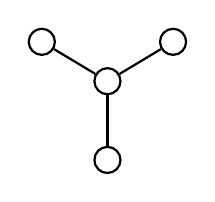
\begin{tikzpicture}[scale=1,
  thick,main node/.style={circle,draw,font=\sffamily\bfseries,minimum size=3mm}]

  \node[main node] (1) at (5/6,1) {};
  \node[main node] (2) at (0,3/2){};
  \node[main node] (3) at (10/6,3/2){};
  \node[main node] (4) at (5/6,0) {};

  \path[every node/.style={font=\sffamily\small}]
   (1) edge node[above]{}(2)
   (1) edge node[above]{}(3)
   (1) edge node[above]{}(4);
\end{tikzpicture}
\end{wrapfigure}
\unhide

Recall that \emph{Alexandrov space} with nonnegative curvature is defined as complete length space with curvature bounded below in the sense of Alexandrov;
the latter is equivalent to the 3-tree comparison; that is, the comparison for the tripod-tree on the diagram. 

Using the introduced notation, a theorem in \cite{AKP} can be restated the following way: \emph{If a complete length-metric space satisfies $3$-tree comparison, then it also satisfies $n$-tree comparison for every positive integer~$n$; in other words it satisfies all monopolar tree comparisons.}

\parbf{Bipolar trees.}
Consider the bipolar trees 3(1) and 2(2) shown on the diagram.

\hide
\begin{center}
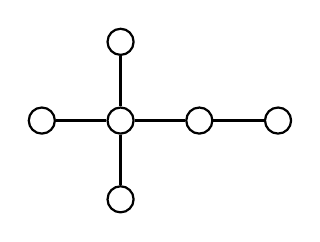
\begin{tikzpicture}[scale=1,
  thick,main node/.style={circle,draw,font=\sffamily\bfseries,minimum size=3mm}]

  \node[main node] (1) at (1,2) {};
  \node[main node] (2) at (1,0){};
  \node[main node] (3) at (1,1){};
  \node[main node] (4) at (0,1) {};
  \node[main node] (5) at (3,1) {};
  \node[main node] (6) at (2,1) {};

  \path[every node/.style={font=\sffamily\small}]
   (1) edge node[above]{}(3)
   (2) edge node[above]{}(3)
   (3) edge node[above]{}(6)
   (4) edge node[above]{}(3)
   (5) edge node[above]{}(6);
\end{tikzpicture}
\hskip30mm
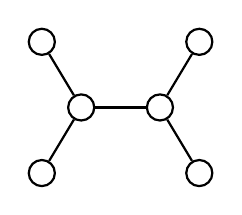
\begin{tikzpicture}[scale=1,
  thick,main node/.style={circle,draw,font=\sffamily\bfseries,minimum size=3mm}]

  \node[main node] (1) at (0,0) {};
  \node[main node] (2) at (1/2,5/6){};
  \node[main node] (3) at (0,10/6){};
  \node[main node] (4) at (2,0) {};
  \node[main node] (5) at (3/2,5/6) {};
  \node[main node] (6) at (2,10/6) {};

  \path[every node/.style={font=\sffamily\small}]
   (1) edge node[above]{}(2)
   (2) edge node[above]{}(3)
   (2) edge node[above]{}(5)
   (4) edge node[above]{}(5)
   (5) edge node[above]{}(6);
\end{tikzpicture}
\end{center}
\unhide
The following theorem is proved in Section~\ref{6-dipole};
it states that the corresponding comparisons also follow form  Alexandrov's comparison.

\begin{thm}{Theorem}\label{thm:3(1)+2(2)}
Any Alexandrov space with nonnegative curvature satisfies  3(1)-tree and 2(2)-tree comparisons.
\end{thm}

\hide
\begin{wrapfigure}{r}{31 mm}
\vskip-2mm
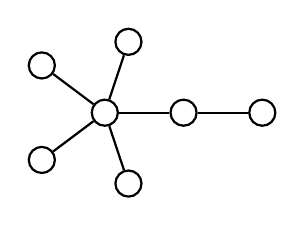
\begin{tikzpicture}[scale=1,
  thick,main node/.style={circle,draw,font=\sffamily\bfseries,minimum size=3mm}]

  \node[main node] (0) at (.3,.9){};
   \node[main node] (1) at (-.8,-.6){};
  \node[main node] (2) at (.3,-.9){};
  \node[main node] (3) at (0,0){};
  \node[main node] (4) at (-.8,.6){};
  \node[main node] (5) at (2,0){};
  \node[main node] (6) at (1,0){};

  \path[every node/.style={font=\sffamily\small}]
     (0) edge node[above]{}(3)
   (1) edge node[above]{}(3)
   (2) edge node[above]{}(3)
   (3) edge node[above]{}(6)
   (4) edge node[above]{}(3)
   (5) edge node[above]{}(6);
\end{tikzpicture}
\end{wrapfigure}
\unhide

The 4(1)-tree comparison turns out to be related to the  so called \emph{transport continuity property}, briefly TCP.
A compact Riemannian manifold $M$ is TCP 
if for any two regular measures with density functions bounded away from zero and infinity the generalized solution of Monge--Amp\`{e}re equation provided by optimal transport 
is a genuine solution.



A necessary condition for TCP was given by Xi-Nan Ma, Neil Trudinger and Xu-Jia Wang in \cite{MTW}.
A key step in the understanding this condition was made by Grégoire Loeper in~\cite{loeper}.
The manifolds satisfying this condition will be called \emph{cost-convex};
using terminology of \cite{MTW+CTIL}, cost-convexity is CTIL+MTW.
Cost-convexity is defined and discussed in Section~\ref{sec:cost-convex}.

\begin{thm}{Theorem}\label{T=>CTIL:CTIL}
If a complete Riemannian manifold satisfies 4(1)-tree comparison, then it is cost-convex; moreover it satisfies all bipolar tree comparisons.
\end{thm}

The two parts of the theorem are proved in sections \ref{7-dipole} and \ref{convexity}.
The proof of the second part works for all complete length spaces (see Corollary \ref{cor:4(1)=>n(1)}).
In this poof, we describe 4(1)-tree comparison using convexity of certain function on the tangent space (see Proposition~\ref{prop:convexity});
we also give an analogous characterization of cost-convex manifolds (see Proposition~\ref{prop:convexity-MTW}).

It is straightforward to check that the spherical 4(1)-tree comparison implies the strict cost-convexity, which in turns implies TCP; see \cite{FRV-Nec+Suf}.

The following question remains open.

\begin{thm}{Question}
Is it true that Rieamnnian manifold is cost-convex if and only if it satisfies 4(1)-tree comparison. 
\end{thm}

From the theorem  above we get that for complete Riemannian manifold satisfying 4(1)-tree comparison also satisfies 3(2)-tree and 3(3)-tree comparisons.
In both cases, the converse is not known.

\parbf{All tree comparisons.}
Finally we consider spaces satisfying \emph{all tree comparisons}.

Recall that a map $f\:W\to X$ between metric spaces is called \emph{submetry} if for any $w\in W$ and $r\ge 0$, we have 
\[f[B(w,r)_W]=B(f(w),r)_X,\]
where $B(w,r)_W$ denotes the ball with center $w$ and radius $r$ in the space $W$.
In other words submetry is a map which is 1-Lipschitz and 1-co-Lipschitz at the same time.
Note that by the definition, any submetry is onto.

\begin{thm}{Theorem}\label{thm:hilbert-quotient}
A separable metric space $X$ satisfies all tree comparisons if and only if
$X$ is isometric to a target space of submetry defined on a subset  of the Hilbert space.
\end{thm}

The following proposition provides a source of examples of spaces satisfying all tree comparisons.
For example, since $\SS^n=\SO(n)/\SO(n-1)$, any round sphere has this property.


\begin{thm}{Proposition}\label{prop:group}
Suppose $G$ is a compact Lie group with bi-invariant metric, so the action $G\times G\acts G$ defined by $(h_1,h_2)\cdot g=h_1\cdot g\cdot  h_2^{-1}$ is isometric. 
Then for any closed subgroup $H<G\times G$, the bi-quotient space $G/\!\!/H$ satisfies all tree comparisons
\end{thm}

From proposition above and Theorem~\ref{T=>CTIL:CTIL}, it follows that the bi-quotient space $G/\!\!/H$ is cost-convex (or equivalently CTIL+MTW), see Section~\ref{sec:cost-convex}.
This makes it closely related to the result of Young-Heon Kim and Robert McCann in \cite{kim-mccann}.

\section{Digressions}

\parbf{On matrix inequality.}
The comparison for monopolar trees has an algebraic corollary which was used Urs Lang and Viktor Schroeder in \cite{LS}, see also \cite{sturm}. 
Namely, given a point array $p,x_1,\dots,x_n$ in a metric space $X$ consider the matrix $M$ with the components 
\[m_{i,j}=\tfrac12\cdot(|x_i-p|^2+|x_j-p|^2-|x_i-x_j|^2).\]
If the tree comparison for $p/x_1,\dots,x_n$ holds, then 
\[\bm{s}\cdot M\cdot \bm{s}^\top\ge 0\]
for any vector $\bm{s}=(s_1,\dots,s_n)$ with nonnegative components.

\hide
\begin{wrapfigure}{r}{22 mm}
\vskip-20mm
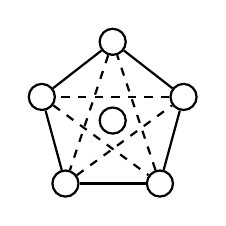
\begin{tikzpicture}[scale=1,
  thick,main node/.style={circle,draw,font=\sffamily\bfseries,minimum size=3mm}, ]

    \node[main node] (0) at (0,0){};
     \node[main node] (1) at (.6,-.8) {};
     \node[main node] (2) at (.9,.3){};
     \node[main node] (3) at (0,1) {};
  \node[main node] (4) at (-.9,.3) {};
  \node[main node] (5) at (-.6,-.8) {};

  \path[every node/.style={font=\sffamily\small}]
  (1) edge node[above]{}(2)
  (2) edge node[above]{}(3)
  (3) edge node[above]{}(4)
  (4) edge node[above]{}(5)
  (5) edge node[above]{}(1)
  (1) edge[dashed] node[above]{}(3)
  (2) edge[dashed] node[above]{}(4)
  (3) edge[dashed] node[above]{}(5)
  (4) edge[dashed] node[above]{}(1)
  (5) edge[dashed] node[above]{}(2);
\end{tikzpicture}
\end{wrapfigure}

However, this condition is not sufficient for the tree comparison for $p/x_1x_2x_3x_4x_5$.
(In general, is not easy to describe tree comparisons using a system of inequalities.)

An example can be constructed by perturbing the configuration on the plane as on the diagram ---
if the diameter of diagram is 1, 
then increasing the distances between the pairs of points connected by dashed lines by $\eps=10^{-9}$ and decreasing  the distances between the pairs of points connected by sold lines by $\delta=10^{-6}$ does the job.
The obtained metric 6-point metric space satisfies the matrix inequality with center at each point, but does not satisfy the tree comparison with pole at the central point.


\parbf{On graph comparison.}
Analogously to the tree comparison one can define graph comparison for any graph by stating that there is model configuration such that the distance between pairs of adjacent points is at most as big and nonadjacent is at least as big.

\begin{thm}{Exercise}
Show that if a graph is a tree, then the graph comparison defined above is equivalent to the tree comparison defined at the beginning of the paper.
\end{thm}


Note that nonnegative and nonpositive curvature can be defined using the comparison for following two graphs on 4 vertexes:

\hide
\begin{center}
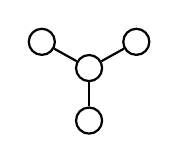
\begin{tikzpicture}[scale=1,
  thick,main node/.style={circle,draw,font=\sffamily\bfseries,minimum size=3mm}]

  \node[main node] (0) at (0,0) {};
  \node[main node] (1) at (-3/5,1/3){};
  \node[main node] (2) at (3/5,1/3){};
  \node[main node] (3) at (0,-2/3) {};

  \path[every node/.style={font=\sffamily\small}]
   (0) edge node[above]{}(1)
   (0) edge node[above]{}(2)
   (0) edge node[above]{}(3);
\end{tikzpicture}
\hskip30mm
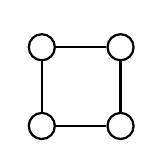
\begin{tikzpicture}[scale=1,
  thick,main node/.style={circle,draw,font=\sffamily\bfseries,minimum size=3mm}]

  \node[main node] (1) at (0,0) {};
  \node[main node] (2) at (0,1){};
  \node[main node] (3) at (1,1){};
  \node[main node] (4) at (1,0) {};

  \path[every node/.style={font=\sffamily\small}]
   (1) edge node[above]{}(2)
   (1) edge node[above]{}(4)
   (2) edge node[above]{}(3)
   (3) edge node[above]{}(4);
\end{tikzpicture}
\end{center}
\unhide

By Reshetnyak majorization theorem,
the nonpositive curvature could be also defined using the comparison for cycle; for example the 6-cycle, the first graph the following diagram.

\hide
\begin{center}
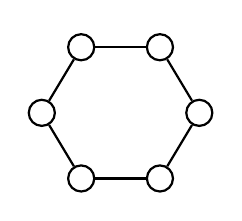
\begin{tikzpicture}[scale=1,
  thick,main node/.style={circle,draw,font=\sffamily\bfseries,minimum size=3mm}]

  \node[main node] (4) at (3/2,5/6){};
   \node[main node] (1) at (1/2,-5/6){};
  \node[main node] (2) at (3/2,-5/6){};
  \node[main node] (0) at (0,0){};
  \node[main node] (5) at (1/2,5/6){};
  \node[main node] (3) at (2,0){};


  \path[every node/.style={font=\sffamily\small}]
    (0) edge node[above]{}(1)
   (1) edge node[above]{}(2)
    (2) edge node[above]{}(3)
   (3) edge node[above]{}(4)
   (4) edge node[above]{}(5)
   (5) edge node[above]{}(0);
\end{tikzpicture}
\hskip30mm
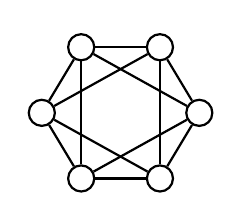
\begin{tikzpicture}[scale=1,
  thick,main node/.style={circle,draw,font=\sffamily\bfseries,minimum size=3mm}]

  \node[main node] (4) at (3/2,5/6){};
   \node[main node] (1) at (1/2,-5/6){};
  \node[main node] (2) at (3/2,-5/6){};
  \node[main node] (0) at (0,0){};
  \node[main node] (5) at (1/2,5/6){};
  \node[main node] (3) at (2,0){};


  \path[every node/.style={font=\sffamily\small}]
    (0) edge node[above]{}(1)
   (1) edge node[above]{}(2)
    (2) edge node[above]{}(3)
   (3) edge node[above]{}(4)
   (4) edge node[above]{}(5)
   (5) edge node[above]{}(0)
    (0) edge node[above]{}(2)
   (1) edge node[above]{}(3)
    (2) edge node[above]{}(4)
   (3) edge node[above]{}(5)
   (4) edge node[above]{}(0)
   (5) edge node[above]{}(1);
\end{tikzpicture}
\end{center}
\unhide

The comparison for the octahedron graph (the second graph on the diagram) implies that the space is nonnegatively curved.
The latter follows since in this graph, a 4-cycle appears as an induced subgraph.
On the other hand, this comparison might be stronger and it might be interesting to understand.

(The tree comparison holds for factors spaces of Hilbert space --- this was the main motivation to consider this type of comparison. 
Unfortunately we do not have analogous examples of nonnegatively curved spaces which would guide us to the right definition.)

\parbf{On colored graph comparison.}
It is also possible to use graph with $(\mp)$-colored edges and define comparison by model configuration such that the distances between vertexes adjacent by a $(-)$-edge does not get larger and by $(+)$-edge does not get smaller.
For example, the $(2{\cdot}n+2)$-comparison (which holds in $\CAT[0]$ length spaces, see \cite{AKP}) can be considered as a comparison for the following colored graph, where $(-)$-edges are marked by solid lines and $(+)$-edges by dashed lines.

\hide
\begin{center}
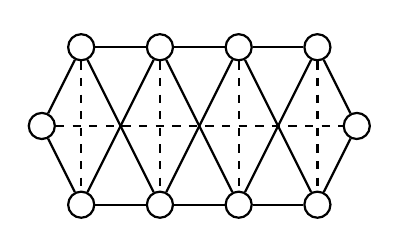
\begin{tikzpicture}[scale=1,
  thick,main node/.style={circle,draw,font=\sffamily\bfseries,minimum size=3mm}]

  \node[main node] (0) at (0.5,0){};
   \node[main node] (1) at (1,1){};
  \node[main node] (2) at (1,-1){};
  \node[main node] (3) at (2,1){};
  \node[main node] (4) at (2,-1){};
  \node[main node] (5) at (3,1){};
\node[main node] (6) at (3,-1){};
 \node[main node] (7) at (4,1){};
\node[main node] (8) at (4,-1){};
\node[main node] (100) at (4.5,0){};

  \path[every node/.style={font=\sffamily\small}]
    (0) edge[dashed] node[above]{}(100)
   (1) edge[dashed] node[above]{}(2)
    (3) edge[dashed] node[above]{}(4)
   (5) edge[dashed] node[above]{}(6)
   (7) edge[dashed] node[above]{}(8)
   (0) edge node[above]{}(1)
   (0) edge node[above]{}(2)
    (1) edge node[above]{}(3)
   (2) edge node[above]{}(4)
   (1) edge node[above]{}(4)
   (2) edge node[above]{}(3)
   (5) edge node[above]{}(3)
   (6) edge node[above]{}(4)
   (5) edge node[above]{}(4)
   (6) edge node[above]{}(3)
   (5) edge node[above]{}(7)
   (6) edge node[above]{}(8)
   (5) edge node[above]{}(8)
   (6) edge node[above]{}(7)
   (7) edge node[above]{}(100)
   (8) edge node[above]{}(100);
\end{tikzpicture}
\end{center}
\unhide
\section{Kirszbraun rigidity}

\begin{thm}{Theorem}\label{thm:kirszbraun-rigid}
Let $A$ be a complete $\CBB[0]$ length space.

Assume that for two point arrays $p,x_1,\dots,x_n\in A$ and $\~q, \~x_1,\dots,\~x_n\in \HH$ we have that 
\[|\~q-\~x_i|\ge |p-x_i|\]
for any $i$,
\[|\~x_i-\~x_j|\le |x_i-x_i|\]
for any pair $(i,j)$
and $\~q$ lies in the interior of the convex hull $K$ of $\~x_1,\dots,\~x_n$.

Then equalities hold in all the inequalities above.
Moreover there is an distance preserving map $f\:K\to A$ such that $f(\~x_i)=x_i$ and $f(\~q)=p$. 
\end{thm}

\parit{Proof.}
By the generalized Kirszbraun theorem, there is a short map $f\:A\to \HH$
such that $f(x_i)=\~x_i$.
Set  $\~p=f(p)$.
By assumptions
\[|\~q-\~x_i|\ge |\~p-\~x_i|.\]

Since $\~q$ lies in the interior of $K$, $\~q=\~p$.
It follows that the equality 
\[|\~q-\~x_i|= |p-x_i|.\]
holds for each $i$.

According to ???, there is a short map $\HH\to \T_p$ such which admits a right inverse $\T_p\to \HH$ such that ...



\qeds
\section{Lower dipolar comparison}

\begin{thm}{Theorem}
Any Alexandrov space with nonnegative curvature satisfies the tree comparison for the following two trees:

\begin{center}
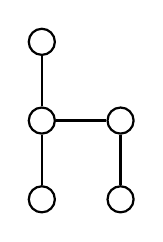
\begin{tikzpicture}[scale=1,
  thick,main node/.style={circle,draw,font=\sffamily\bfseries,minimum size=3mm}]
  \node[main node] (1) at (0,0) {};
  \node[main node] (2) at (0,1){};
  \node[main node] (3) at (0,2){};
  \node[main node] (4) at (1,0) {};
  \node[main node] (5) at (1,1) {};
  

  \path[every node/.style={font=\sffamily\small}]
   (1) edge node[above]{}(2)
   (2) edge node[above]{}(3)
   (2) edge node[above]{}(5)
   (4) edge node[above]{}(5);
\end{tikzpicture}
\hskip10mm
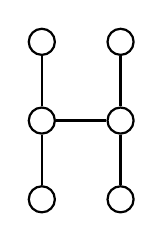
\begin{tikzpicture}[scale=1,
  thick,main node/.style={circle,draw,font=\sffamily\bfseries,minimum size=3mm}]

  \node[main node] (1) at (0,0) {};
  \node[main node] (2) at (0,1){};
  \node[main node] (3) at (0,2){};
  \node[main node] (4) at (1,0) {};
  \node[main node] (5) at (1,1) {};
  \node[main node] (6) at (1,2) {};

  \path[every node/.style={font=\sffamily\small}]
   (1) edge node[above]{}(2)
   (2) edge node[above]{}(3)
   (2) edge node[above]{}(5)
   (4) edge node[above]{}(5)
   (5) edge node[above]{}(6);
\end{tikzpicture}
\hskip10mm
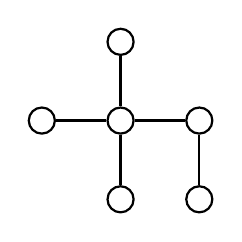
\begin{tikzpicture}[scale=1,
  thick,main node/.style={circle,draw,font=\sffamily\bfseries,minimum size=3mm}]

  \node[main node] (1) at (0,1) {};
  \node[main node] (2) at (1,0){};
  \node[main node] (3) at (1,1){};
  \node[main node] (4) at (1,2) {};
  \node[main node] (5) at (2,0) {};
  \node[main node] (6) at (2,1) {};

  \path[every node/.style={font=\sffamily\small}]
   (1) edge node[above]{}(3)
   (2) edge node[above]{}(3)
   (3) edge node[above]{}(6)
   (4) edge node[above]{}(3)
   (5) edge node[above]{}(6);
\end{tikzpicture}
\end{center}

\end{thm}

\parit{Proof.} First we will show the statement for the first tree and use this in the proofs for the second and third trees.
The latter two proofs are neraly identical.

Let us label the poles by $p_1$ and $p_2$ and the reaming 3 vertexes by $x_1,x_2,x_3$.

The required model configuration $\~p_1$, $\~p_2$, $\~x_1$, $\~x_2$, $\~x_3\in \RR^3$ will be found among the configurations where in addition the angle between $[\~p_1,\~p_2]$ and the remaining edges $[p_j,x_j]$ of the tree are the same as the corresponding angles in $A$; these type of configurations will be called \emph{pivotal}.

Up to a motion of the space, the configuration of that type is completely described by 6 angles $\alpha_{i,j}$ between the planes $\~p_1 \~p_2 \~x_i$ and $\~p_1\~p_2 \~x_j$.

Denote by $\beta_{i,j}$ the minimal angle between the planes $\~p_1 \~p_2 \~x_i$ and $p_1p_2 x_j$ such that $|\~x_i-\~x_j|_{\RR^3}\ge|\~x_i-\~x_j|_A$. 
Note that the configuration $\~p_1,\~p_2,\~x_1,\~x_2,\~x_3,\~x_4$ is valid if $\alpha_{i,j}\ge \beta_{i,j}$ for all pairs $(i,j)$.

Note that $\beta_{i,j}\le \pi$ for any pair $(i,j)$.

In other words, we need to show that if $\~p_1,\~p_2,\~x_i,\~x_j$ is a model configuration with $\alpha_{i,j}=\pi$ then 
\[|\~x_i-\~x_j|_{\RR^3}\ge |x_i-x_j|_{A}.\eqlbl{|x-x|}\]
Note that in this configuration the line segment $[\~x_i,\~x_j]$ intersects the line $\~p_1\~p_2$;
denote by $\~z$ the point of intersection.

If $\~z\in [\~p_1,\~p_2]$, consider the corresponding point $z\in [p_1,p_2]$.
In the remaining case, $\~z\notin [\~p_1,\~p_2]$, without loss of generality, we can assume that $\~z$ lies on the half line $\~p_1\~p_2$.
In this set $z$ to be the image of $p_2$ for the $(\tfrac12\cdot \dist_{p_1}^2)$-gradient flow of $p_2$ for time $t=\ln \tfrac{|\~z-\~p_1|}{|\~p_2-\~p_1|}$.
In both cases the comparsison implies 
\begin{align*}
|x_i-z|_A &\le |\~x_i-\~z|_{\RR^3},
&
|x_j-z|_A &\le |\~x_j-\~z|_{\RR^3}.
\end{align*}
From the triangle inequality, \ref{|x-x|}
follows.

Along the same lines we can show that 
\[\beta_{i,j}+\beta_{j,k}+\beta_{k,i}\le 2\cdot \pi\eqlbl{sum=<2pi}\] 
for any triple $(i,j,k)$.


Indeed, assume contrary.
Since $\beta_{i,k}\le \pi$, it follows that 
\[\beta_{i,j}+\beta_{j,k}> \pi.\eqlbl{sum>=pi}\] 
Consider a configuration $\~p_1,\~p_2,\~x_i,\~x_j,\~x_k\in\RR^3$ such that 
$\alpha_{i,j}=\beta_{i,j}$, $\alpha_{j,k}=\beta_{j,k}$ and the points $x_i$ and $x_k$ lie on the opposite sides from the plane $\~p_1\~p_2\~x_j$.
By \ref{sum>=pi}, $[\~x_i\~x_j\~x_k]$ intersects the line $\~p_1\~p_2$;
denote by $\~z$ the point of intersection.

Let us construct a point $z\in A$ which corresponds to $\~z$ the same way as above.
By construction 
\begin{align*}
|x_i-x_j|_A &= |\~x_i-\~x_j|_{\RR^3},
&
|x_j-x_k|_A &\le |\~x_j-\~x_k|_{\RR^3}.
\end{align*}
By comparison implies 
\begin{align*}
|x_i-z|_A &\le |\~x_i-\~z|_{\RR^3},
&
|x_j-z|_A &\le |\~x_j-\~z|_{\RR^3},
&
|x_k-z|_A &\le |\~x_k-\~z|_{\RR^3}.
\end{align*}
By comparison, 
\[|x_i-x_k|_A \le  |\~x_i-\~x_k|_{\RR^3};\]
hence \ref{sum=<2pi} follows.


Assume one of the triangle inequalities 
\[\beta_{i,k}\le \beta_{i,j}+\beta_{j,k}\]
does not hold.
Order the values $\{\beta_{i,j}\}$ in a nonincreasing order.
Let us construct a metric graph with 4 vertexes labeled by $\{1,2,3,4\}$
the following way choose the the largest value $\beta_{i,j}$ 
and attche an edge $(i,j)$ of length $\beta_{i,j}$,
do the same for the second largest value and so on,
starting from third step, before adding new edge we have to check that the triangle inequalities does not brake; in other words we want to 
At the end we get a metric 
\qeds
\section{Pull-back convexity}\label{convexity}

In this section reformulate 4(1)-tree comparison using convexity of certain function on tangent space and use it to prove the second part of Theorem \ref{T=>CTIL:CTIL}.

\begin{thm}{Proposition}\label{prop:convexity}
If a Riemannian manifold $M$ satisfies $4(1)$-tree comparison then it is CTIL and the for any $p,q\in M$ the function $f\: \TIL_p\to \RR$ defined by
\[f(v)=\tfrac12\cdot\dist_q^2\circ\exp_p(v)-\tfrac12\cdot|v|^2\] 
is concave.

Converse also holds; moreover, if $f$ is convex for any $p,q\in M$ then $M$ satisfies all bipolar trees comparisons; that is the $m(n)$-tree comparison for any $m$ and $n$.
\end{thm}



Recall that for a continuous function $f$ defined on metric space we write 
$f''\le \lambda$ if for any unit-speed geodesic $\gamma$ the function
\[t\mapsto f\circ\gamma(t)-\lambda\cdot \tfrac{t^2}{2}\]
is a concave real-to-real function.

\parit{Proof.}
Assume $M$ satisfies 4(1)-tree comparison.
Since 4(1)-tree comparison implies 3-tree comparison,
$M$ has nonnegative sectional curvature.

Fix $u,v\in \TIL_p$ and $w\in [u,v]$.
Assume that $g\:[u,v]\:\RR$ is the function which is uniquely defined by conditions:
\[g''=1,\quad
g(u)=f(u)\quad
\text{and}\quad
g(w)=f(w).\]
It is sufficient to show that $g(v)\ge f(v)$.

Fix small $\eps>0$ and set
\begin{align*}
x&=\exp_p u, 
&y&=\exp_p v, 
&z&=\exp_pw,
\\
x'&=\exp_p(-\eps\cdot  u),
&y'&=\exp_p(-\eps\cdot  v)
\end{align*}
Apply the $p/xyx'y'(z/q)$ comparison and pass to the limit as $\eps\to 0$.
We obtain a configuration of points $\~p, \~x, \~y, \~z, \~q\in\HH$, satisfying corresponding comparisons and
such that
\begin{align*}
\measuredangle[\~p\,^{\~x}_{\~y}]&= \measuredangle[p\,^{x}_{y}],
&\measuredangle[\~p\,^{\~x}_{\~z}]&= \measuredangle[p\,^{x}_{z}],
&\measuredangle[\~p\,^{\~z}_{\~y}]&= \measuredangle[p\,^{z}_{y}].
\end{align*}
In particular,
from above and Toponogov comparison, we have
\begin{align*}
|\~x-\~y|_\HH&=|u-v|_{\T_p},
&|\~z-\~y|_\HH&=|w-v|_{\T_p},
&|\~x-\~z|_\HH&=|u-w|_{\T_p},
\\
|\~q-\~z|_\HH&=|q-z|_M,
&|\~q-\~x|_\HH&\ge|q-x|_M,
&|\~q-\~y|_\HH&\ge|q-y|_M.
\end{align*}

Let $q^*\in \HH$ be the point
such that 
\begin{align*}
|q^*-\~z|&=|q-z|, 
&|q^*-\~x|&=|q-x|
\end{align*}

Assume
$\varphi\:[u,v]_{\T_p}\to[\~x,\~y]_{\HH}$ is an isometry such that
$\varphi(u)=\~x$, $\varphi(v)=\~y$ and
$\varphi(w)=\~z$.
Then $g:=\dist^2_{q^*}\circ\varphi$, indeed, we have, that $g''=1$ and
$$g(u)=|q^*-\~x|^2=|q-x|^2=f(u),\quad
g(w)=|q^*-\~z|^2=|q-z|^2=f(w)$$
$$g(v)=|q^*-\~y|^2=|q-y|^2\ge f(u).$$
Hence the statement.

\parit{Converse.}
Fix points $p$ and $q$ in $M$;
set $\~q=\log_pq\in\T_p$.
Note that 
\[f\le \~f,\eqlbl{eq:f=<f}\] 
where 
\[\~f(v)=\tfrac12\cdot |v-\~q|_{\T_p}^2-\tfrac12\cdot |v|_{\T_p}^2.\]
Further note that the inequality \ref{eq:f=<f} is equivalent to the Toponogov comparison for all hinges $[p\,{}^x_q]$ in $M$.
It follows that $M$ has nonnegative sectional curvature. 

\medskip

Now fix a bipolar geodesic tree $[p/x_1\dots x_n(q/y_1\dots y_m)]$ in $M$.
Set 
\[\~p=0=\log_pp,\quad \~q=\log_pq,\quad\text{and}\quad \~x_i=\log_px_i\]
for each $i$. 

Consider the linear map $\psi\:\T_q\to \T_p$ such that for any smooth function $h$
\[\psi_1\:\nabla_{q}h\mapsto \nabla_{\~q}(h\circ\exp_p).\]
Since sectional curvature of $M$ is nonnegative, the restriction $\exp_p|_{\TIL_p}$ is short and therefore $\psi_1$ is short.

In particular there is a linear map $\psi_2\:\T_q\to\T_p$ such that, the map $\iota\:\T_q\zz\to \T_p\oplus\T_p$ defined by
\[\iota\:v\mapsto \psi_1(v)\oplus \psi_2(v)\]
is distance preserving.

Further set 
\[h_i=\tfrac12\cdot\dist_{y_i}^2
\quad
f_i=h_i\circ\exp_p|_{\TIL_p}
\quad
\~y_i=\~q-\zeta(\nabla_q h_i).
\]


By construction
\[|\~y_i-\~q|_{\T_p\oplus\T_p}=|y_i-q|_M.\]

At the point $\~q$ the restriction functions $\~f_i=\tfrac12\cdot\dist^2_{\~w}|_{\T_p}$ and the function $f_i$ have the same value and gradient.
Since $f_i''\le 1$ and $\~f_i''=1$, we get $\~f_i\ge f_i$. 
The latter implies
\[
|\~y_i-\~p|_{\T_p\oplus\T_p}\ge|y_i-p|_M
\quad
\text{and}
\quad
|\~y_i-\~x_j|_{\T_p\oplus\T_p}\ge|y_i-x_j|_M.\]
for any $i$ and $j$.

Since $\T_p\oplus\T_p$ admits an isometric embedding into the Hilbert space,
we get the needed configuration.
\qeds

The Plaut's theorem makes possible to extend the proof above to complete length spaces;
that is, we get the following corollary from the proof.

\begin{thm}{Corollary}\label{cor:4(1)=>n(1)}
If a complete length space $X$ satisfies $4(1)$-tree comparison then it satisfies any bipolar tree comparisons.
\end{thm}

For MTW manifolds we have somewhat weaker statement.

\begin{thm}{Proposition}\label{prop:convexity}
A CTIL Riemannian manifold $M$ is MTW if and only if 
for any $p,q\in M$ the function $f\: \TIL_p\to \RR$ defined by
\[f(v)=\tfrac12\cdot(\dist_q^2\circ\exp_p(v)-|v|^2)\] 
has convex suplevel sets.
\end{thm}
\section{MTW}\label{MTW+}


Proposition~\ref{MTW-plus-convexity} provides equivalence of (\textit{\ref{thm:convexity:convexity}}) and (\textit{\ref{thm:convexity:MTW}}) in the main theorem (\ref{thm:convexity}); which is the final step its proof.
The equivalence is proved by calculations along the same lines as in \cite[Chapter 12]{villani}.

Let us introduce notations and use them to reformulate the property (\textit{\ref{thm:convexity:MTW}}).

\parbf{Tangent vectors.}
Let $M$ be a Riemannian manifold, $p\in M$.
Denote by $\IL_p$ the \emph{inner locus} of $p$; it can be defined as the $\exp_p$-image of $\TIL_p$ or, equivalently, as the complement $M\backslash \CL_p$, where $\CL_p$ denotes the cut locus of $p$.
Note that $q\in\IL_p$ if and only if $p\in \IL_p$.

Assume $q\in\IL_p$; that is, $q=\exp_pW$ for some $W\zz\in \TIL_p M$.
Given a vector $Y\in T_q$, consider the unique vector $Y_p\in\T_p$ such that 
\[Y=(d_W\exp_p)Y_p.\]

Note that $p=\exp_q(-W_q)$ if $p$, $q$ and $W$ are as above.

Given $x\in\IL_p$ such that $x=\exp_pX$ for some  $X\in \TIL_p$,  set
\[\tilde Y_p(x)=(d_X\exp_p) Y_p;\]
this way we defined a vector field $\tilde Y_p$ in $\IL_p$.

Note that in the vector field $\tilde Y_p$ is constant in the normal coordinates at $p$;
in particular 
\[\nabla_X\tilde Y_p=0\eqlbl{eq:zero}\] 
for any $X\in\T_p$.
Further, note that 
\[Y\tilde Y_pf=Y\tilde Y_qf+(\nabla_Y\tilde Y_p)f\eqlbl{eq:nabla}\]
for $Y\in \T_q$ and any smooth function $f$.
Indeed applying \ref{eq:zero}, we get that
\begin{align*}
(Y\tilde Y_p-Y\tilde Y_q)f
&=[(\tilde Y_q\tilde Y_p-\tilde Y_p\tilde Y_q)f](q)=
\\
&=(\nabla_Y \tilde Y_p-\nabla_Y\tilde Y_q)f=\nabla_Y \tilde Y_pf.
\end{align*}


\parbf{Column notation.} Given two points $p$ and $q$ in a Riemannian manifold $M$,
let us define the cost function $(p,q)\mapsto \cost{p}{q}$ as
\[\dcost{}{}{p}{q}=\tfrac12\cdot|p-q|^2_M\]
We will need to differentiate the cost function by both argument.
In order to avoid possible confusion, we will write the vector next to the differentiated argument. 
For example
\[\dcost{X}{Y}{p}{q}\]
is the second mixed derivative of the cost function at the pair $(p,q)$, once by the first argument ($p$) along the vector $X \in \T_p$ and once by the second argument ($q$) along the vector field $Y\in \T_q$.
We may also write a vector field instead of the vectors.

Using the introduced notations,
we can reformulate the property (\textit{\ref{thm:convexity:MTW}}) in Theorem~\ref{thm:convexity}
as

\begin{itemize}
 \item[\textit{(ii)}$'$] \emph{If $X\in \T_p$, $Y\in\T_q$ and $q\in \IL_p$, then
 \[\dcost{X\tilde X_p}{Y\tilde Y_p}{p}{q}\le 0.\]}
\end{itemize}

The left hand side of the last inequality, multiplied by $(-\tfrac32)$ is called \emph{MTW-curvature} or \emph{cost-curvature}; it is denoted by $\mathfrak{S}(X,Y)$, see \cite[equation 12.21]{villani};
if $p=q$, then $\mathfrak{S}(X,Y)$ coincides with the curvature $\langle\Rm(X,Y)Y,X\rangle$, see \cite[12.30]{villani}.
In particular, if the condition (\textit{\ref{thm:convexity:MTW}}) holds, then the manifold has nonnegative sectional curvature. 


Assume $q=\exp_pW$ for some $W\in\TIL_p$. 
Then 
\[\dcost{X}{{}}{p}{q}=-\langle X,W\rangle;\eqlbl{derX}\]
\[\dcost{X}{Y}{p}{q}=-\langle X,Y_p\rangle =-\langle X_q,Y\rangle\eqlbl{derXY}\]
and
\[\dcost{X}{Y\tilde Y_p}{p}{q}=0.\eqlbl{derXYY}\]

Indeed, \ref{derX} is equivalent to the first variation formula.
Taking the derivative of \ref{derX} in the normal coordinates at $p$ we get \ref{derXY}.
\[\dcost{X}{Y}{p}{q}=-\langle X,Y_p\rangle.\]
Since $q\in \IL_p$ if and only if $p\in\IL_q$ we can swap $p$ and $q$ and get the second identity in \ref{derXY}. Finally, the value $\langle X,Y_p\rangle$ does not depend on $q$; therefore the derivative along the second argument \ref{derXY} has to vanish;
hence \ref{derXYY} follows.

Let us use the identities to show that 
\[\dcost{X\tilde X_p}{Y\tilde Y_p}{p}{q}=\dcost{X\tilde X_p}{Y\tilde Y_p}{p}{q}
\quad
\text{or, equivalently}
\quad
\mathfrak{S}(X,Y)=\mathfrak{S}(Y,X).\eqlbl{derXXYY}\]
This identity will not be used in the sequel, but it might help the reader to adapt to the column notation.

Applying \ref{eq:nabla}, we get that
\begin{align*}
\dcost{X\tilde X_p}{Y\tilde Y_p}{p}{q}&=\dcost{X\tilde X_p}{Y\tilde Y_q}{p}{q}+\dcost{X\tilde X_p}{\nabla_Y\tilde Y_q}{p}{q}=
\\
&=\dcost{X\tilde X_p}{Y\tilde Y_q}{p}{q}+\dcost{X\tilde X_q}{\nabla_Y\tilde Y_q}{p}{q}-\dcost{\nabla_X\tilde X_p}{\nabla_Y\tilde Y_q}{p}{q}.
\end{align*}
By \ref{derXYY}, 
\[\dcost{X\tilde X_q}{\nabla_Y\tilde Y_q}{p}{q}=0.\]
Therefore
\[\dcost{X\tilde X_p}{Y\tilde Y_p}{p}{q}=\dcost{X\tilde X_p}{Y\tilde Y_q}{p}{q}-\dcost{\nabla_X\tilde X_p}{\nabla_Y\tilde Y_q}{p}{q}.\]
The right hand side is symmetric in $p$ and $q$;
hence \ref{derXXYY} follows.

\begin{thm}{Proposition}\label{MTW-plus-convexity}
Let $M$ be a CTIL Riemannian manifold.
Then the following conditions are equivalent:
\begin{enumerate}[(a)]
 \item\label{MTW-plus-convexity:MTW} For any $p\in M$, $q\in \IL_p$, $X\in \T_p$ and $Y\in\T_q$ we have
 \[\dcost{X\tilde X_p}{Y\tilde Y_p}{p}{q}\le 0.\]
 \item\label{MTW-plus-convexity:h} For any $p_0,p_1\in M$, the function $h\:\TIL_{p_0}\to\RR$ defined by
\[h(X)=\cost{{p_1}}{\exp_{p_0}X}-\cost{{p_0}}{\exp_{p_0}X}\]
is concave;
 \item\label{MTW-plus-convexity:f}  For any $p_0,p_1\in M$, the function $f\:\TIL_{p_0}\to\RR$ defined by
\[f(X)=\cost{p_1}{\exp_{p_0}X}\]
is 1-concave.
\end{enumerate}
\end{thm}


Note that equivalence 
(\textit{\ref{MTW-plus-convexity:MTW}})$\iff$(\textit{\ref{MTW-plus-convexity:f}}) imply the
equivalence of (\textit{\ref{thm:convexity:convexity}})$\iff$(\textit{\ref{thm:convexity:MTW}}) in \ref{thm:convexity}. 
Therefore the proposition finishes the proof of the main theorem.


\parit{Proof.}  
Note that $\cost{p_0}{\exp_{p_0}X}=\tfrac12\cdot |X|^2$ for any $X\in\TIL_{p_0}$,
in particular the function $s(X)\zz=\cost{p_0}{\exp_{p_0}X}$ is $1$-affine (that is, $1$-concave and $1$-convex at the same time).

Evidently $f=h+s$, therefore (\textit{\ref{MTW-plus-convexity:h}})$\iff$(\textit{\ref{MTW-plus-convexity:f}}).



\parit{(\ref{MTW-plus-convexity:MTW}) $\Rightarrow$ (\ref{MTW-plus-convexity:h}).}
Note that the function $h$ is semiconcave.
Therefore $h$ is concave if
\[\tfrac{d^2}{dt^2}h(U+t\cdot V)\le 0\]
at $t=0$ for almost all vectors $U\in\TIL_p$ and $V\in \T_p$.

Using the column notation, we can rewrite the inequality in the following equivalent form:
\[
\begin{matrix}{{}}\\{Y\tilde Y_{p_0}}
\end{matrix}
\left(\dcost{}{}{p_1}{q}-\dcost{}{}{p_0}{q}\right)\le 0\eqlbl{eq:MTW-plus}\]
for any $p_0,p_1, q$ and $Y\in \T_q$;
from above it is sufficient to prove \ref{eq:MTW-plus} for almost all $q$; in particular, we can assume that $p_0,p_1\in \IL_q$.

Let $W, X\in \TIL_q$ be such that $p_0=\exp_qW$, $p_1=\exp_q(W+X)$.
Since $M$ is CTIL, $W+t\cdot X\in\TIL_q$ for any $t\in[0,1]$;
set $p_t=\exp_q(W+t\cdot X)$.


Let us use the identity
$f(1)-f(0)-f'(0)=\int_0^1f''(t)\cdot(1-t)\cdot dt$,
for the function 
\[f(t)=\dcost{}{Y\tilde Y_{q}}{p_t}{q};\]
Note that
\[f'(0)=\dcost{X}{Y\tilde Y_{q}}{p_0}{q}
\quad
\text{and}
\quad 
f''(t)
=\dcost{\tilde X_{q}\tilde X_{q}}{Y\tilde Y_{q}}{p_t}{q},\]
therefore
\[\dcost{}{Y\tilde Y_{q}}{p_1}{q}-\dcost{}{Y\tilde Y_{q}}{p_0}{q}-\dcost{X}{Y\tilde Y_{q}}{p_0}{q}=\int_0^1 \dcost{\tilde X_{q}\tilde X_{q}}{Y\tilde Y_{q}}{p_t}{q}\cdot dt.\]

By (\textit{\ref{MTW-plus-convexity:MTW}}), the term under the integral is nonpositive; therefore
\[
\dcost{{}}{Y\tilde Y_{q}}{}{}
\left(\dcost{}{}{p_1}{q}-\dcost{}{}{p_0}{q}\right)
\le
\dcost{X}{Y\tilde Y_{q}}{p_0}{q}.\]
By \ref{eq:nabla}, we can rewrite the last inequality the following way:
\[
\dcost{{}}{Y\tilde Y_{p_0}}{}{}
\left(\dcost{}{}{p_1}{q}-\dcost{}{}{p_0}{q}\right)
\le
\dcost{{}}{\nabla_Y \tilde Y_{p_0}}{}{}
\left(\dcost{}{}{p_1}{q}
-
\dcost{}{}{p_0}{q}\right)
+
\dcost{X}{Y\tilde Y_{q}}{p_0}{q}.
\eqlbl{eq:MTW-plus-extra}\]

Applying \ref{derX}, we get that
\begin{align*}
\dcost{{}}{\nabla_Y \tilde Y_{p_0}}{}{}
\left(\dcost{}{}{p_1}{q}
-
\dcost{}{}{p_0}{q}\right)
&=
-\langle\nabla_Y \tilde Y_{p_0},W+X\rangle + \langle\nabla_Y \tilde Y_{p_0},W\rangle
=
\\
&=-\langle\nabla_Y \tilde Y_{p_0},X\rangle.
\end{align*}
Further, applying \ref{derXYY} and \ref{derXY}, we get that
\begin{align*}
\dcost{X}{Y\tilde Y_{q}}{p_0}{q}
&=
\dcost{X}{Y\tilde Y_{p_0}}{p_0}{q}-\dcost{X}{\nabla_Y\tilde Y_{p_0}}{p_0}{q}=
\\
&=0+\langle\nabla_Y \tilde Y_{p_0},X\rangle.
\end{align*}
It follows that the right hand side in \ref{eq:MTW-plus-extra} vanishes;
hence \ref{eq:MTW-plus} follows.

\parit{(\ref{MTW-plus-convexity:h}) $\Rightarrow$ (\ref{MTW-plus-convexity:MTW}).}
Let $p_t$, $q$, $W$, $X$ and $Y$ be as above;
set 
\[h_t(Z)=\cost{{p_t}}{\exp_{p_0}Z}-\cost{{p_0}}{\exp_{p_0}Z}.\]
Note that $h_0\equiv 0$; in particular 
\[Y\tilde Y_{p_0}h_0=0\]
for any $Y\in\T_q$.

By (\textit{\ref{MTW-plus-convexity:h}}), 
\[Y\tilde Y_{p_0}h_t\le 0.\]
It follows that 
\[\frac{d^2}{dt^2}(Y\tilde Y_{p_0}h_t)\le 0\]
at $t=0$.
Finally note that 
\[\dcost{X\tilde X_{p_0}}{Y\tilde Y_{p_0}}{p_0}{q}=\frac{d^2}{dt^2}(Y\tilde Y_{p_0}h_t);\]
hence the part (\textit{\ref{MTW-plus-convexity:h}}) follows.
\qeds


\section{All tree comparisons}\label{sec:all-tree}


\parit{Proof of Theorem~\ref{thm:hilbert-quotient}.}
The ``if'' part is left as an exercise;
let us prove the ``only if'' part.

Fix a point array $a_1,\dots, a_n$ in $X$.
Consider the complete graph $K_n$ with the vertexes labeled by $a_1,\dots, a_n$.


Let $\hat K_n\to K_n$ be the universal covering.
Denote by $\hat  V$ the set of vertexes of $\hat  K_n$;
given a vertex $\hat  v\in\hat V$ denote by $v$ the corresponding vertex of $K_n$.

Applying the tree comparison for finite subtrees in $\hat  K_n$ and passing to a partial limit,  we get the following:

\begin{enumerate}[$({*})$]
\item There is a map $f\:\hat V\to\HH$ such that 
\[|f(\hat v)-f(\hat w)|_\HH\ge |v-w|_X\]
for any two vertexes $\hat v,\hat w\in \hat  V$ and the equality holds if $(\hat v,\hat w)$ is an edge in $\hat  K_n$.
\end{enumerate}

For $Y=f(\hat V)$ the projection $Y\to X$ defined by $f(\hat v)\mapsto v$ is the required submetry.
It finishes the proof if $X$ is finite.

Since $X$ is separable, it has a countable everywhere dense set $\{a_1,a_2,\dots\}$. 
Applying the statement above for $X_n=\{a_1,\dots a_n\}$, we get 
a submetry from $Y_n=f_n(\hat V_n)\subset \HH$ to $X_n$.

It remains to pass to the ulralimit $Y$ of the subspaces $Y_n$.
Clearly $Y$ admits an isometric embedding into $\HH$ 
and it admits submetry on $Y\to X$.
Hence the statement follows.
\qeds


The following proof was suggested by Alexander Lytchak, it is simplified version of the construction of Chuu-Lian Terng and Gudlaugur Thorbergsson given in \cite[Section 4]{terng-thorbergsson}.


\parit{Proof of Proposition~\ref{prop:group}.}
Denote by $G^n$ the direct product of $n$ copies of $G$.
Consider the map $\phi_n\:G^n\to G/\!\!/H$ defined by
\[\phi_n\:(\alpha_1,\dots,\alpha_n)\mapsto [\alpha_1\cdots\alpha_n]_H,\]
where $[x]_H$ denotes the $H$-orbit of $x$ in $G$.

Note that $\phi_n$ is a quotient map for the action of $H\times G^{n-1}$ on $G^n$ defined by
\[(\beta_0,\dots,\beta_n)\cdot(\alpha_1,\dots,\alpha_n)=(\gamma_1\cdot \alpha_1\cdot\beta_1^{-1},\beta_1\cdot\alpha_2\cdot\beta_2^{-1},\dots,\beta_{n-1}\cdot\alpha_n\cdot\beta_n^{-1}),\]
where $\beta_i\in G$ and $(\beta_0,\beta_n)\in H<G\times G$. 

Denote by $\rho_n$ the product metric on $G^n$ rescaled with factor $\sqrt{n}$.
Note that the quotient $(G^n,\rho_n)/(H\times G^{n-1})$ is isometric to $G/\!\!/H=(G,\rho_1)/\!\!/H$.

As $n\to\infty$ the curvature of $(G^n,\rho_n)$ converges to zero and its injectivity radius goes to infinity.
Therefore passing to the ultra-limit of $G^n$ as $n\to\infty$ we get the Hilbert space.
It remains to observe that the limit action has the required property.
\qeds

\section{Final remarks}

The following problem discussed in \cite[7.1]{AKP} was one of the original motivations to study the tree comparison.

\begin{thm}{Problem}
Which finite metric spaces admit isometric embeddings into Alexandrov spaces with curvature $\ge \kappa$.
\end{thm}

The problem is still open.
According to \cite[4.1]{AKP}, the $n$-tree comparison provides a necessary condition for the problem.
This condition is sufficient for the 4-point metric spaces and possibly for 5-point metric spaces, but not sufficient for 6-point metric spaces.
The corresponding example of 6-point metric space was constructed by Sergei Ivanov, see \cite{AKP}.

Theorem~\ref{2(2)+3(1)}, provides a source for such examples --- it is sufficient to construct construct 6-pint metric space which satisfy all 5-tree comparisons, but does not satisfy 2(2)-tree comparison.
This class of examples includes the example of Sergei Ivanov;
it does not satisfies the comparison for $y/az(q/xb)$ in the notations of \cite[7.1]{AKP}.

We expect that the 5-tree and 2(2)-tree comparisons (see the trees on the diagram) are sufficient for 6-point metric spaces. 
\hide
\begin{center}
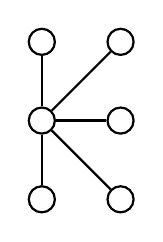
\begin{tikzpicture}[scale=1,
  thick,main node/.style={circle,draw,font=\sffamily\bfseries,minimum size=3mm}]

  \node[main node] (1) at (0,0) {};
  \node[main node] (2) at (0,1){};
  \node[main node] (3) at (0,2){};
  \node[main node] (4) at (1,0) {};
  \node[main node] (5) at (1,1) {};
  \node[main node] (6) at (1,2) {};

  \path[every node/.style={font=\sffamily\small}]
   (1) edge node[above]{}(2)
   (2) edge node[above]{}(3)
   (2) edge node[above]{}(4)
   (2) edge node[above]{}(5)
   (2) edge node[above]{}(6);
\end{tikzpicture}
\hskip10mm
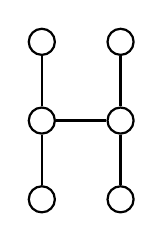
\begin{tikzpicture}[scale=1,
  thick,main node/.style={circle,draw,font=\sffamily\bfseries,minimum size=3mm}]

  \node[main node] (1) at (0,0) {};
  \node[main node] (2) at (0,1){};
  \node[main node] (3) at (0,2){};
  \node[main node] (4) at (1,0) {};
  \node[main node] (5) at (1,1) {};
  \node[main node] (6) at (1,2) {};

  \path[every node/.style={font=\sffamily\small}]
   (1) edge node[above]{}(2)
   (2) edge node[above]{}(3)
   (2) edge node[above]{}(5)
   (5) edge node[above]{}(6)
   (4) edge node[above]{}(5);
\end{tikzpicture}
\end{center}
\unhide




\begin{thebibliography}{52}
\bibitem{AKP} S. Alexander, V. Kapovitch, A. Petrunin, 
\emph{Alexandrov meets Kirszbraun.} 
Proceedings of the Gökova Geometry-Topology Conference 2010, 88--109, Int. Press, Somerville, MA, 2011.

%\bibitem{AKP-book} S. Alexander, V. Kapovitch, and A. Petrunin, \emph{Alexandrov geometry.} book in preparation.

%\bibitem{berg-nikolaev} Berg, I. D.; Nikolaev, I. G., \emph{Quasilinearization and curvature of Aleksandrov spaces.} Geom. Dedicata 133 (2008), 195--218.


\bibitem{FRV-Nec+Suf} Figalli, A.; Rifford, L.; Villani, C.,
\emph{Necessary and sufficient conditions for continuity of optimal transport maps on Riemannian manifolds.} Tohoku Math. J. (2) 63 (2011)

\bibitem{karcher}
Karcher, H.,
\emph{Schnittort und konvexe Mengen in vollständigen Riemannschen Mannigfaltigkeiten.}
Math. Ann. 177 1968 105--121.

\bibitem{kim-mccann} Kim, Y.-H.; McCann, R.,
\emph{Towards the smoothness of optimal maps on Riemannian submersions and Riemannian products (of round spheres in particular).}
J. Reine Angew. Math. 664 (2012), 1--27. 

\bibitem{LS}  Lang, U.; Schroeder, V.,
\emph{Kirszbraun's theorem and metric spaces of bounded curvature.}
Geom. Funct. Anal. 7 (1997), no. 3, 535–560. 

\bibitem{lebedeva-petrunin} Lebedeva, N., Petrunin, A., \emph{Curvature bounded below: a definition a la Berg--Nikolaev.} Electron. Res. Announc. Math. Sci. 17 (2010), 122--124.

\bibitem{loeper}
Loeper, G.,
\emph{On the regularity of solutions of optimal transportation problems.}
Acta Math. 202 (2009), no. 2, 241–283. 

\bibitem{MTW}  Ma, X.-N.; Trudinger, N.  Wang, X.-J.,
\emph{Regularity of potential functions of the optimal transportation problem.}
Arch. Ration. Mech. Anal. 177 (2005), no. 2, 151--183. 

\bibitem{naor}  Naor, A., \emph{An introduction to the Ribe program.} Jpn. J. Math., 7(2):167--233, 2012.

\bibitem{ohta}  Ohta, S.-I.,
\emph{Markov type of Alexandrov spaces of non-negative curvature.} Mathematika, 55(1-2):177--189, 2009.

\bibitem{petrunin} Petrunin, A., \emph{In search of a five-point Alexandrov type condition.}  St. Petersburg Math. J. 29 (2018), no. 1.

\bibitem{perelman-petrunin} Perelman, G.; Petrunin, A., \emph{Extremal subsets in Aleksandrov spaces and the generalized Liberman theorem.} St. Petersburg Math. J. 5 (1994), no. 1, 215--227.

%\bibitem{sato} Sato, T., \emph{An alternative proof of Berg and Nikolaev’s characterization of CAT(0)-spaces via quadrilateral inequality.} Arch. Math. (Basel), 93(5):  487--490, 2009.

\bibitem{sturm}  Sturm, K. T., \emph{Metric spaces of lower bounded curvature.} Exposition. Math., 17(1):35–47, 1999.


\bibitem{terng-thorbergsson}  Terng, C.-L.,  Thorbergsson, G.
\emph{Submanifold geometry in symmetric spaces.} J. Differential Geom. 42 (1995), no. 3, 665--718.

\bibitem{MTW+CTIL+} Villani, C., \emph{Regularity of optimal transport and cut locus: from nonsmooth analysis to geometry to smooth analysis.} Discrete Contin. Dyn. Syst. 30 (2011), no. 2, 559–571. 
 
\bibitem{MTW+CTIL} Villani, C., \emph{Stability of a 4th-order curvature condition arising in optimal transport theory.}
J. Funct. Anal. 255 (2008), no. 9, 2683--2708.

 
\bibitem{villani}  Villani, C. \emph{Optimal transport. Old and new.} Grundlehren der Mathematischen Wissenschaften 338. Springer-Verlag, Berlin, 2009.
\end{thebibliography}


%\section{Seven point comparison}\label{7-dipole}

Let $M$ be a Riemannian manifold.
The \emph{tangent injectivity locus} at the point $p\in M$ (briefly $\TIL_p$) is defined as the maximal open subset in the tangent space $\T_p$ such that for any $v\in\TIL_p$ the geodesic path $\gamma(t)=\exp_p(v\cdot t)$, $t\in [0,1]$ is a minimizing.
If the tangent injectivity locus at any point $p\in M$ is convex we say that $M$ satisfies \emph{convexity of  tangent injectivity locus} or briefly $M$ is CTIL.

Xi-Nan Ma, Neil Trudinger and Xu-Jia Wang, Xu-Jia introduced a global differential geometric condition which is now called MTW, see \cite{MTW}.
The conditions CTIL and MTW are necessary for the regularity of optimal transport on Riemannian manifold $M$.
Moreover, a slightly stronger version of these conditions gives the converse.

{
\hide
\begin{wrapfigure}[6]{r}{24 mm}
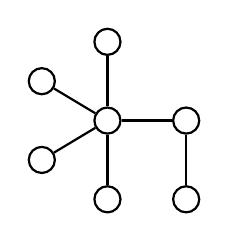
\begin{tikzpicture}[scale=1,
  thick,main node/.style={circle,draw,font=\sffamily\bfseries,minimum size=3mm}]

  \node[main node] (0) at (1/6,1/2) {};
   \node[main node] (1) at (1/6,3/2) {};
  \node[main node] (2) at (1,0){};
  \node[main node] (3) at (1,1){};
  \node[main node] (4) at (1,2) {};
  \node[main node] (5) at (2,0) {};
  \node[main node] (6) at (2,1) {};

  \path[every node/.style={font=\sffamily\small}]
     (0) edge node[above]{}(3)
   (1) edge node[above]{}(3)
   (2) edge node[above]{}(3)
   (3) edge node[above]{}(6)
   (4) edge node[above]{}(3)
   (5) edge node[above]{}(6);
\end{tikzpicture}
\end{wrapfigure}
\unhide

\begin{thm}{Proposition}\label{T=>CTIL+MTW}
Let $T$ be the tree as on the diagram.
If a Riemannian manifold $M$ satisfies the $T$-tree comparison then 
\begin{enumerate}[(a)]
\item\label{T=>CTIL:CTIL} $M$ is CTIL;
\item\label{T=>CTIL:MTW} $M$ is MTW.
\end{enumerate}

\end{thm}

In the proof we will use a reformulation of MTW condition
given by Cédric Villani \cite[2.6]{MTW+CTIL}.
More precisely, we will use the following reformulation of which can be proved the same way.

}

Assume $u,v\in \T_p$ and $w=\tfrac12\cdot(u+v)$
and $x=\exp_p u$, $y=\exp_pv$ and $q=\exp_pw$.
If the three geodesic paths $[p,x]$, $[p,y]$ and $[p,q]$ described by the paths 
$t\mapsto\exp_p(t\cdot u)$,  $t\mapsto\exp_p(t\cdot v)$, $t\mapsto\exp_p(t\cdot w)$ for $t\in[0,1]$ are minimizing, then $[p,q]$ is called \emph{median} of the hinge $[p\,^x_y]$.
Note that in a CTIL Riemannian manifold, any hinge has a median.

\begin{thm}{MTW condition}\label{MTW}
Assume $M$ be a CTIL Riemannian manifold. 
Then $M$ is MTW if and only if for a median $[p,q]$ of any hinge $[p\,^x_y]$ one of the following inequalities
\[
\left[
\begin{aligned}
|p-q|^2_M-|z-q|^2_M&\le |p-x|^2_M-|z-x|^2_M,
\\
|p-q|^2_M-|z-q|^2_M&\le |p-y|^2_M-|z-y|^2_M.
\end{aligned}
\right.
\]
holds for any $z\in M$.
\end{thm}

\parit{Proof; (\ref{T=>CTIL:CTIL}).}
Assume the contrary; that is, there is $p\in M$ and $u,v\zz\in \TIL_p$ such that $w=\tfrac12\cdot(u+v)\notin \TIL_p$.

Let $\tau$ be the maximal value such that the geodesic $\gamma(t)=\exp_p(w\cdot t)$ is a length-minimizing on $[0,\tau]$.
Set $w'=\tau\cdot w$.
Note that $\tau<1$ and $w'\in\partial \TIL_p$.


Set $q=\exp_p w'$.
By general position argument, we can assume that there are at least two minimizing geodesics connecting $p$ to $q$; see \cite{karcher}.
That is, there is $w''\in \partial \TIL_p$ such that $w''\ne w'$ and $\exp_pw'=\exp_pw''$.

\begin{center}
\begin{lpic}[t(-0 mm),b(-0 mm),r(0 mm),l(0 mm)]{pics/7-config(1)}
\lbl[r]{1.5,32;$x$}
\lbl[l]{59.5,31;$y$}
\lbl[t]{18.5,2;$y'$}
\lbl[t]{32.5,2;$x'$}
\lbl[t]{26,4.5;$p$}
\lbl[r]{22.5,16;$z$}
\lbl[r]{25,32;$q$}
\lbl[l]{28.5,27;$q'$}
\end{lpic}
\end{center}

Fix small positive real numbers $\delta,\eps$ and $\zeta$.
Consider the points
\begin{align*}
q'=q'(\eps)&=\exp_p(1-\eps)\cdot w',
&
z=z(\zeta)&=\exp_p(\zeta\cdot w''),
\\
x&=\exp_p u,
&
x'=x'(\delta)&=\exp_p (-\delta\cdot u),
\\
y&=\exp_p v,
&
y'=y'(\delta)&=\exp_p (-\delta\cdot v).
\end{align*}
We will  show that for some choice of $\delta,\eps$ and $\zeta$ the array $p,x,x',y,y',q',z$ does not satisfy the $T$-tree comparison with the labeling as on the diagram below.

\hide
\begin{wrapfigure}[7]{r}{26 mm}
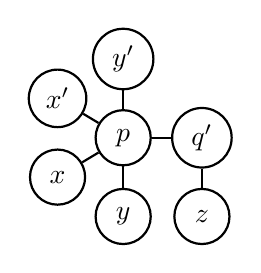
\begin{tikzpicture}[scale=1,
  thick,main node/.style={circle,draw,font=\sffamily\bfseries,minimum size=7mm}]

  \node[main node] (0) at (1/6,1/2) {$x$};
   \node[main node] (1) at (1/6,3/2) {$x'$};
  \node[main node] (2) at (1,0){$y$};
  \node[main node] (3) at (1,1){$p$};
  \node[main node] (4) at (1,2) {$y'$};
  \node[main node] (5) at (2,0) {$z$};
  \node[main node] (6) at (2,1) {$q'$};

  \path[every node/.style={font=\sffamily\small}]
     (0) edge node[above]{}(3)
   (1) edge node[above]{}(3)
   (2) edge node[above]{}(3)
   (3) edge node[above]{}(6)
   (4) edge node[above]{}(3)
   (5) edge node[above]{}(6);
\end{tikzpicture}
\end{wrapfigure}
\unhide

Assume that given  positive numbers $\delta,\eps$ and $\zeta$, there is a point array $\~p$, $\~x$, $\~x'(\delta)$, $\~y$, $\~y'(\delta)$, $\~q'(\eps)$, $\~z(\zeta)\in\HH$ as in the definition of $T$-tree comparison;
that is, the distances between the points in this array are at least as big as the distances of corresponding points in $M$ and the equality holds for the pair adjacent in $T$.

Since $\delta$ is small, we can assume that $p$ lies on a necessary unique minimizing geodesic $[x,x']_M$.
Hence 
\[|x-x'|_M=|x-p|_M+|p-x'|_M.\]
By comparison
\begin{align*}
|\~x-\~x'|_\HH&\ge|x-x'|_M,
\\
|\~x-\~p|_\HH&=|x-p|_M,
\\
|\~x'-\~p|_\HH&=|x'-p|_M.
\end{align*}
By triangle inequality,
\[|\~x-\~x'|_\HH=|\~x-\~p|_\HH+|\~x'-\~p|_\HH;\]
that is, $\~p\in [\~x,\~x']_\HH$.
The same way we see that $\~p\in [\~y,\~y']_\HH$.

Fix $\eps$ and $\zeta$.
Note that as $\delta\to 0$ we have 
\begin{align*}
\~x'&\to \~p,
&
\~y'&\to \~p.
\\
\measuredangle[\~p\,^{\~x'}_{\~y}]&\to \measuredangle[p\,^{x'}_{y}],
&
\measuredangle[\~p\,^{\~y'}_{\~x}]&\to \measuredangle[p\,^{y'}_{x}],
\\
\measuredangle[\~p\,^{\~x'}_{\~q'}]&\to \measuredangle[p\,^{x'}_{q'}],
&
\measuredangle[\~p\,^{\~y'}_{\~q'}]&\to \measuredangle[p\,^{y'}_{q'}],
\end{align*}
It follows that 
\begin{align*}
\measuredangle[\~p\,^{\~x}_{\~y}]&\to \measuredangle[p\,^x_y],
&
\measuredangle[\~p\,^{\~x}_{\~q'}]&\to \measuredangle[p\,^x_{q'}],
&
\measuredangle[\~p\,^{\~y}_{\~q'}]&\to \measuredangle[p\,^y_{q'}].
\end{align*}


Therefore, passing to a partial limit as $\delta\to0$, we get a configuration of 5 points 
$\~p, \~x,\~y,\~q'=\~q'(\eps),\~z=\~z(\zeta)$ such that  
\begin{align*}
\measuredangle[\~p\,^{\~x}_{\~y}]&= \measuredangle[p\,^{x}_{y}],
&
\measuredangle[\~p\,^{\~y}_{\~q'}]&= \measuredangle[p\,^{y}_{q'}],
&
\measuredangle[\~p\,^{\~x}_{\~q'}]&= \measuredangle[p\,^{x}_{q'}].
\end{align*}
In other words, the map sending 4 points $0,u,v,w'\in\T_p$ to $\~p,\~x,\~y,\~q\in\HH$ correspondingly is distance preserving.

Note that $q'\to q$ as $\eps\to0$. 
Therefore, in the limit,
we get a configuration $\~p$, $\~x$, $\~y$, $\~q'$, $\~z=\~z(\zeta)$ such that in addition we have
\begin{align*}
|\~q'-\~z|&=|q-z|,
&
|\~p-\~z|&\ge |p-z|,
\\
|\~x-\~z|&\ge |x-p|,
&
|\~y-\~z|&\ge |y-z|
\end{align*}

Since $w''\ne w'$, for small values $\zeta$ the last three inequalities 
imply 
\[|\~q'-\~z|>|q-z|,\]
a contradiction.





\parit{(\ref{T=>CTIL:MTW}).}
Fix a hinge $[p\,^x_y]$ in $M$.
By \textit{(\ref{T=>CTIL:CTIL})}, $M$ is CTIL.
Therefor $[p\,^x_y]$ has a median; denote it by $[p,q]$.
For $\delta>0$, define $x'=x'(\delta)$ and $y'=y'(\delta)$ as above.

\hide
\begin{wrapfigure}{r}{26 mm}
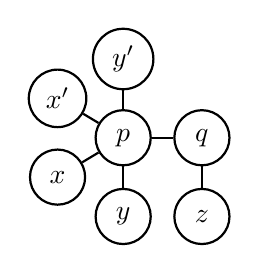
\begin{tikzpicture}[scale=1,
  thick,main node/.style={circle,draw,font=\sffamily\bfseries,minimum size=7mm}]

  \node[main node] (0) at (1/6,1/2) {$x$};
   \node[main node] (1) at (1/6,3/2) {$x'$};
  \node[main node] (2) at (1,0){$y$};
  \node[main node] (3) at (1,1){$p$};
  \node[main node] (4) at (1,2) {$y'$};
  \node[main node] (5) at (2,0) {$z$};
  \node[main node] (6) at (2,1) {$q$};

  \path[every node/.style={font=\sffamily\small}]
     (0) edge node[above]{}(3)
   (1) edge node[above]{}(3)
   (2) edge node[above]{}(3)
   (3) edge node[above]{}(6)
   (4) edge node[above]{}(3)
   (5) edge node[above]{}(6);
\end{tikzpicture}
\end{wrapfigure}
\unhide

Without loss of generality we can assume that $x,y\zz\in\exp_p(\TIL_p)$.
If $\delta$ is small, the latter implies that $p$ lies on unique minimizing geodesics $[x,x']$ and $[y,y']$.

Consider a limit case $T$-tree comparison as $\delta\to 0$;
we get a configuration of 5 points $\~p$, $\~q$, $\~x$, $\~y$ and $\~z$ such that
\begin{align*}
\measuredangle[\~p\,^{\~x}_{\~y}]&=\measuredangle[p\,^x_y],
\end{align*}
$\~q$ is the midpoint of $[\~x, \~y]$.
In particular,
\begin{align*}
2\cdot|\~z-\~q|_\HH^2+|\~q-\~x|_\HH^2+|\~q-\~y|_\HH^2
&=
|\~z-\~x|_\HH^2+|\~z-\~y|_\HH^2,
\\
2\cdot|\~p-\~q|_\HH^2+|\~q-\~x|_\HH^2+|\~q-\~y|_\HH^2
&=
|\~p-\~x|_\HH^2+|\~p-\~y|_\HH^2,
\end{align*}

By the comparison,
\begin{align*}
|\~z-\~x|_\HH&\ge |z-x|_M,
&
|\~z-\~y|_\HH&\ge |z-y|_M,
\\
|\~p-\~x|_\HH&\ge |p-x|_M,
&
|\~p-\~y|_\HH&\ge |p-y|_M,
\\
|\~q-\~x|_\HH&= |q-x|_M,
&
|\~q-\~y|_\HH&= |q-y|_M,
\\
|\~q-\~z|_\HH&= |q-z|_M,
&
|\~q-\~p|_\HH&= |q-p|_M,
\end{align*}
Therefore
\begin{align*}
2\cdot|z-q|_M^2+|q-x|_M^2+|q-y|_M^2
&\ge
|z-x|_M^2+|z-y|_M^2,
\\
2\cdot|p-q|_M^2+|q-x|_M^2+|q-y|_M^2
&\le
|p-x|_M^2+|p-y|_M^2.
\end{align*}
Hence the condition in \ref{MTW} follows.
\qeds



\Addresses
\end{document}
